\documentclass[twocolumn,10pt]{asme2ej}

\usepackage{epsfig} 

\title{Gesichtserstellung mittels GANs}

\author{Tobias Rohrer
    \affiliation{
	Hochschule Darmstadt\\
	Data Science (Master)\\
    Email: sttorohr@stud.h-da.de
    }	
}

\graphicspath{ {./images/} }
\usepackage[center]{caption}
\usepackage[locale=DE]{siunitx}
\usepackage{hyperref}

\usepackage{listings}
\usepackage{xcolor}

\definecolor{codegreen}{rgb}{0,0.6,0}
\definecolor{codegray}{rgb}{0.5,0.5,0.5}
\definecolor{codepurple}{rgb}{0.58,0,0.82}
\definecolor{backcolour}{rgb}{0.95,0.95,0.92}

\lstdefinestyle{mystyle}{
	backgroundcolor=\color{backcolour},   
	commentstyle=\color{codegreen},
	keywordstyle=\color{magenta},
	numberstyle=\tiny\color{codegray},
	stringstyle=\color{codepurple},
	basicstyle=\ttfamily\footnotesize,
	breakatwhitespace=false,         
	breaklines=true,                 
	captionpos=b,                    
	keepspaces=true,                 
	numbers=left,                    
	numbersep=5pt,                  
	showspaces=false,                
	showstringspaces=false,
	showtabs=false,                  
	tabsize=2
}
\lstset{style=mystyle}
\begin{document}

\maketitle    

%%%%%%%%%%%%%%%%%%%%%%%%%%%%%%%%%%%%%%%%%%%%%%%%%%%%%%%%%%%%%%%%%%%%%%
\begin{abstract}
{\it In der vorliegenden Arbeit wurde ein Deep Convolutional Generative Adversarial Network (DCGAN) zur Erstellung von Gesichtern erstellt. Das DCGAN wurde mit Hilfe des CelebA-Datensatzes trainiert. Für die Implementierung wurden die state-of-the-art TensorFlow 2 und TensorFlow Dataset APIs verwendet.
}
\end{abstract}

%%%%%%%%%%%%%%%%%%%%%%%%%%%%%%%%%%%%%%%%%%%%%%%%%%%%%%%%%%%%%%%%%%%%%%
\section{Einleitung}
Generative Adversarial Networks (GANs) \cite{goodfellow2014generative} sind laut einer der Gründerväter der Convolutional Neural Networks, Yann LeCun: \begin{quote}
"the most interesting idea in the last 10 years in Machine Learning"
\end{quote}
GANs sind generative Modelle, die es ermöglichen aus zufälligen Eingabewerten neue Daten zu erstellen, die den Trainingsdaten ähneln. DCGANs sind eine Unterkategorie von GANs, welche sich an Convolutional Neural Networks (CNNs) orientieren und eine tiefe Netzwerkarchitektur, sowie Faltungen implementieren. Heute werden GANs und DCGANs unter anderem verwendet, um die Auflösung von Bildern zu erhöhen, Bilder zu restaurieren oder auch um neue Trainingsdaten zum trainieren von tiefen neuronalen Netzen zu erstellen. Das Ziel der vorliegenden Arbeit ist die Implementierung eines DCGANs zur Erstellung von Bildern mit menschlichen Gesichtern. Als Vorbild für das Vorhaben diente die Website \url{www.thispersonoesnotexist.com}. Das in dieser Arbeit entworfene und implementierte DCGAN orientiert sich an den Architektur-Richtlinien aus \cite{radford2015unsupervised}.

\section{Generative Adversarial Networks}
Die Idee der GANs wurde 2014 in \cite{goodfellow2014generative} präsentiert. Ein GAN besteht aus einem generativen Model $G$ und einem diskriminierendem Model $D$. Hierbei ist $D$ ein Klassifizierer mit der Aufgabe, echte Trainingsdaten $X_{train}$ von den durch $G$ erstellten Daten $X_{gen}$ zu unterscheiden.  Das Model $G$ hat das Ziel, neue Daten ($X_{gen}$) zu erstellen, die nicht von $D$ von echten Trainingsdaten unterschieden werden können. Das Training von $D$ und $G$ erfolgt simultan, wobei die Modelle sich gegenseitig versuchen auszuspielen.

\section{Konzeption}\label{sec:2}

\begin{figure}
	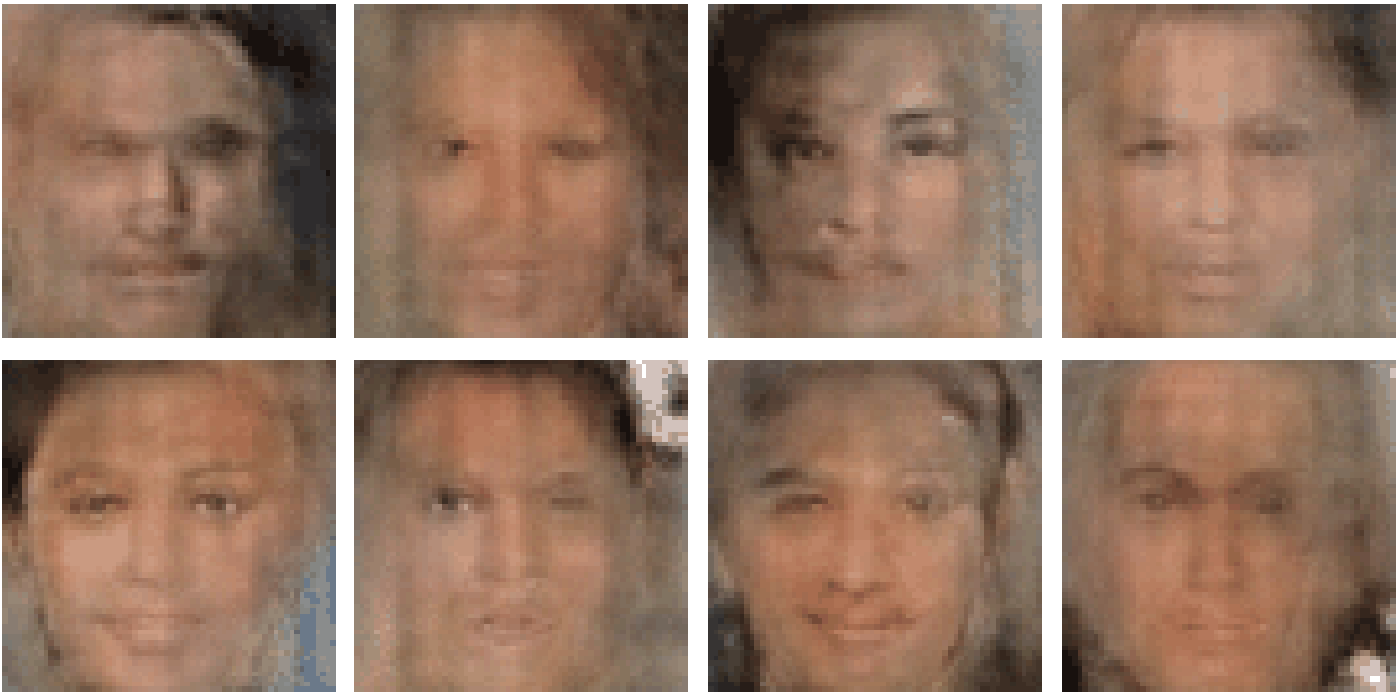
\includegraphics[scale=0.35	]{result.png}
	\caption[center]{Gesichter, die durch den Generator nach dem Training erstellt wurden.}
	\label{fig:result}
\end{figure}

Zum Trainieren des Diskriminators $D$ wurde der Large-scale CelebFaces Attributes (CelebA) Datensatz verwendet \cite{liu2015faceattributes}. CelebA enthält insgesamt 202.599 Bilder von 10.177 Identitäten. Um den Rechenaufwand gering zu halten, wurde eine zufällige Teilmenge von 50.000 Bildern verwendet. Die Daten durchlaufen vor dem Training mehrere Vorbereitungsschritte. Zum einen wird aus dem Zentrum des Bildes das Gesicht herausgeschnitten um unnötige Hintergrunddetails zu entfernen. Zum anderen werden alle Bilder auf eine einheitliche Größe von 64x64x3 Pixeln runterskaliert. Das Ergebnis eines Vorbereitungsschrittes wird in Abbildung \ref{fig:preprocessing} veranschaulicht. Die Architektur des GAN, bestehend aus $G$ und $D$, ist in den Abbildungen \ref{fig:disc} und \ref{fig:gen} skizziert. 

\begin{figure}[h]
	\centering
	\captionsetup{justification=centering}
	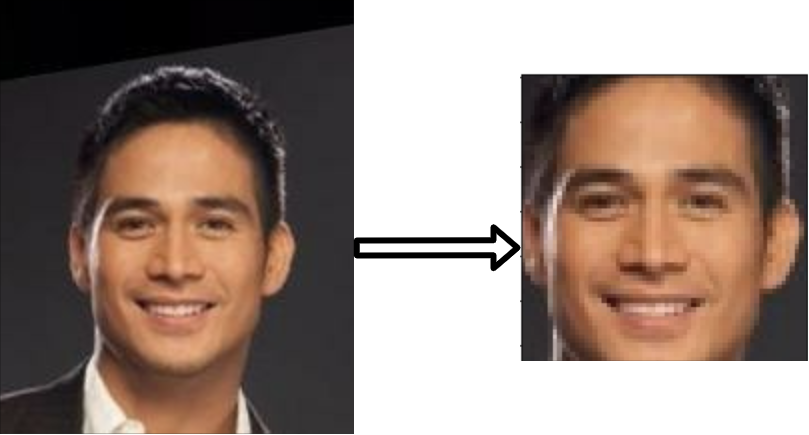
\includegraphics[scale=0.2]{preprocessing.png}
	\caption[center]{Bild als Original (links) und nach der Vorverarbeitung (rechts)}
	\label{fig:preprocessing}
\end{figure}
\newpage
\subsection{Diskriminator}
Der Diskriminator $D$ besteht aus 2 Faltungsschichten, sowie einer voll vernetzen Schicht zur Klassifizierung. Die Faltungsschichten arbeiten mit 5x5 großen Faltungskernen und einer Schrittweite von 2. Wie in \cite{radford2015unsupervised} als Teil der Richtlinie für GAN-Architekturen vorgeschlagen, werden somit die \emph{Pooling-Schichten} durch die Schrittweite der Faltungskerne ersetzt. Als Eingabe erwartet der $D$ einen Datensatz mit den Dimensionen 64x64x3. Die Ausgabe des Diskriminators ist ein Skalar $o \in \left[ 0 ; 1  \right]$, wobei $o \leq 0.5$ einer Klassifikation als unecht, also vom GAN erzeugt, und $o > 0.5$ einer Klassifikation als echt, also vom Trainingsdatensatz, entspricht.
\begin{figure}[h]
	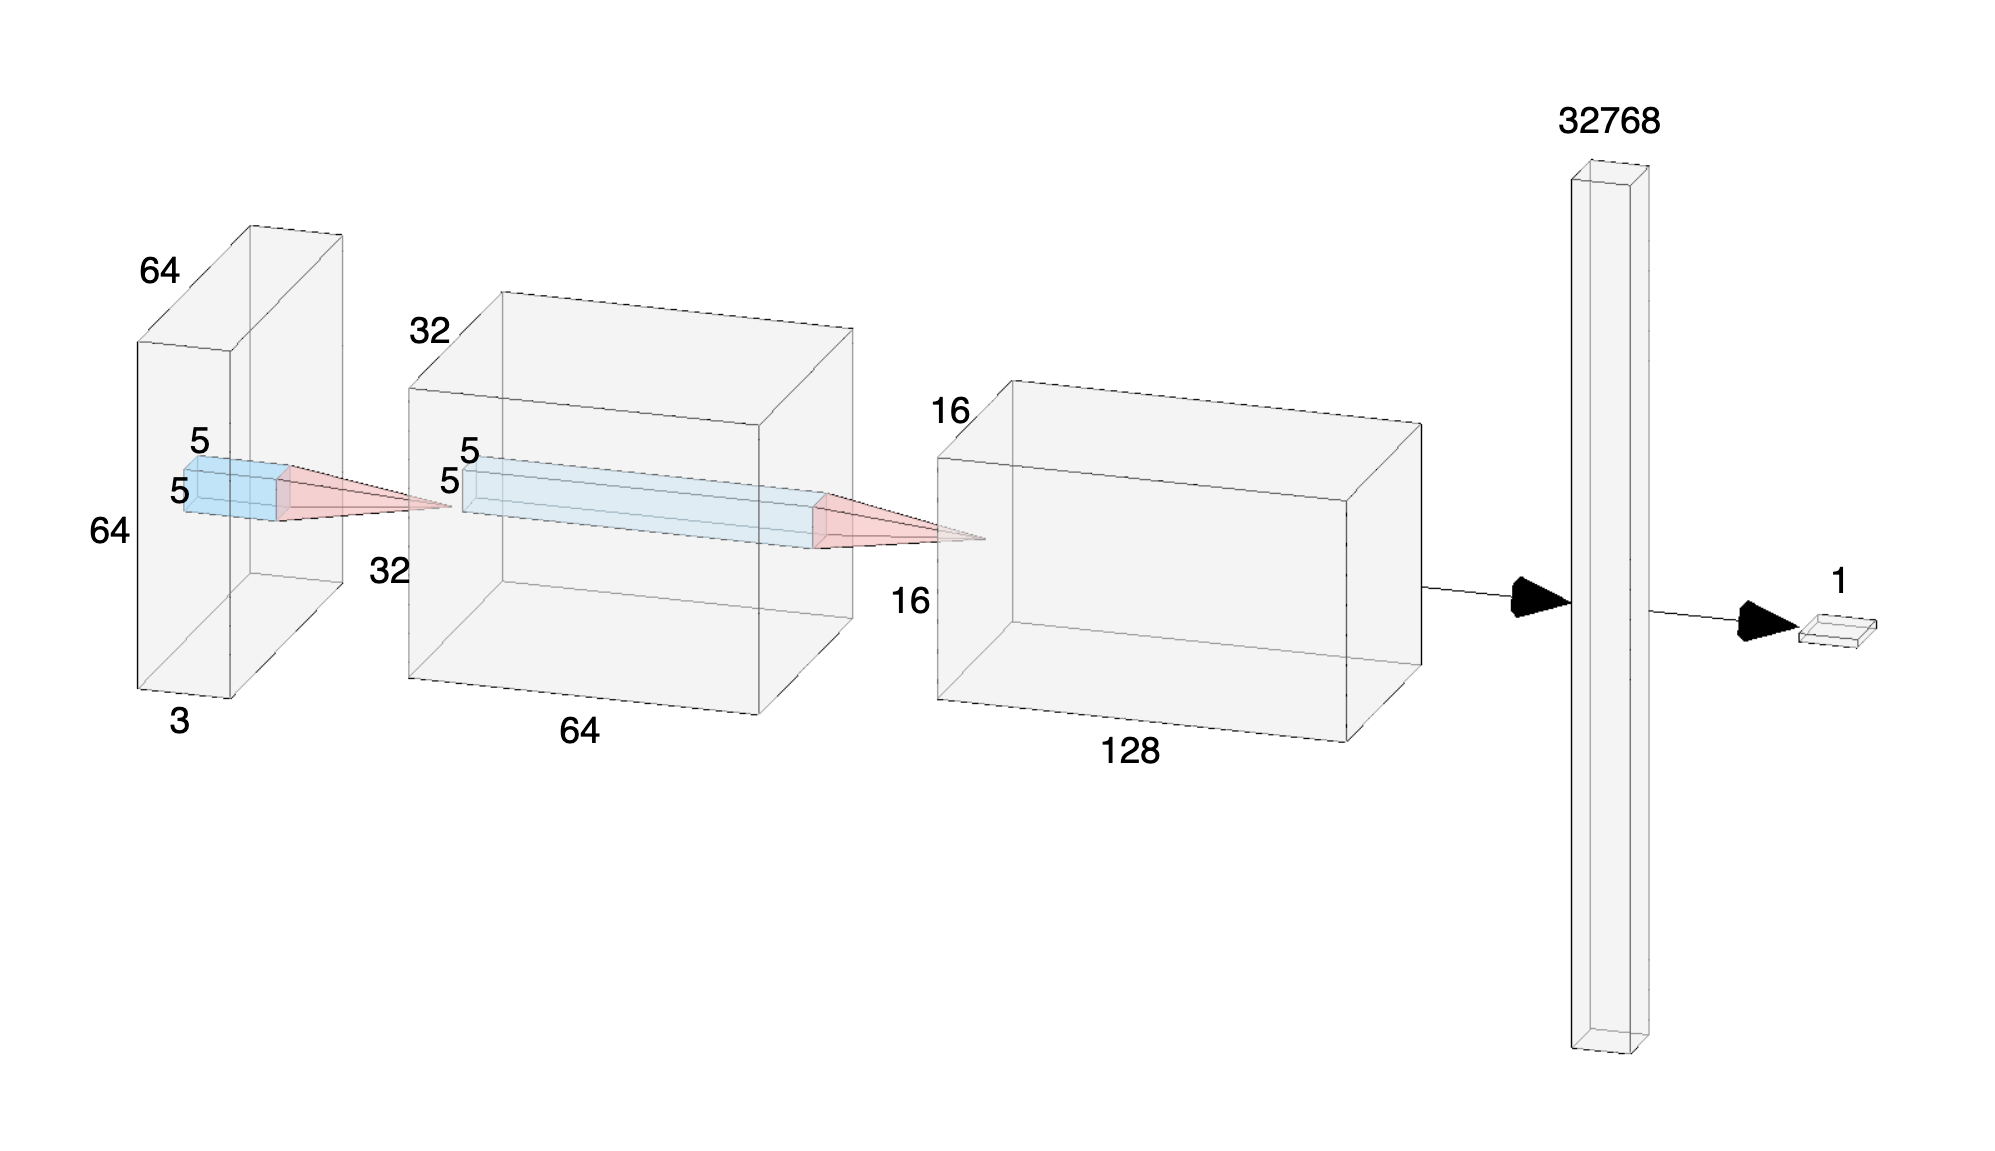
\includegraphics[scale=0.12]{disc.png}
	\caption[center]{Architektur des Diskriminators $D$}
	\label{fig:disc}
\end{figure}

\subsection{Generator}
Die Eingabeschicht des Generator $G$ mit der Dimension 100x1 nimmt einen Vektor $X_{random}$ mit zufälligen Werten, die aus einer Standardnormalverteilung gezogen wurden, entgegen. Über eine voll vernetzte Schicht folgen drei Schichten, die eine transponierte Faltung implementieren. Analog zu $D$ werden Faltungskerne der Größe 5x5 eingesetzt. Die Ausgabe von $G$ ist ein Bild mit den Dimensionen 64x64x3.
\begin{figure}[h]
	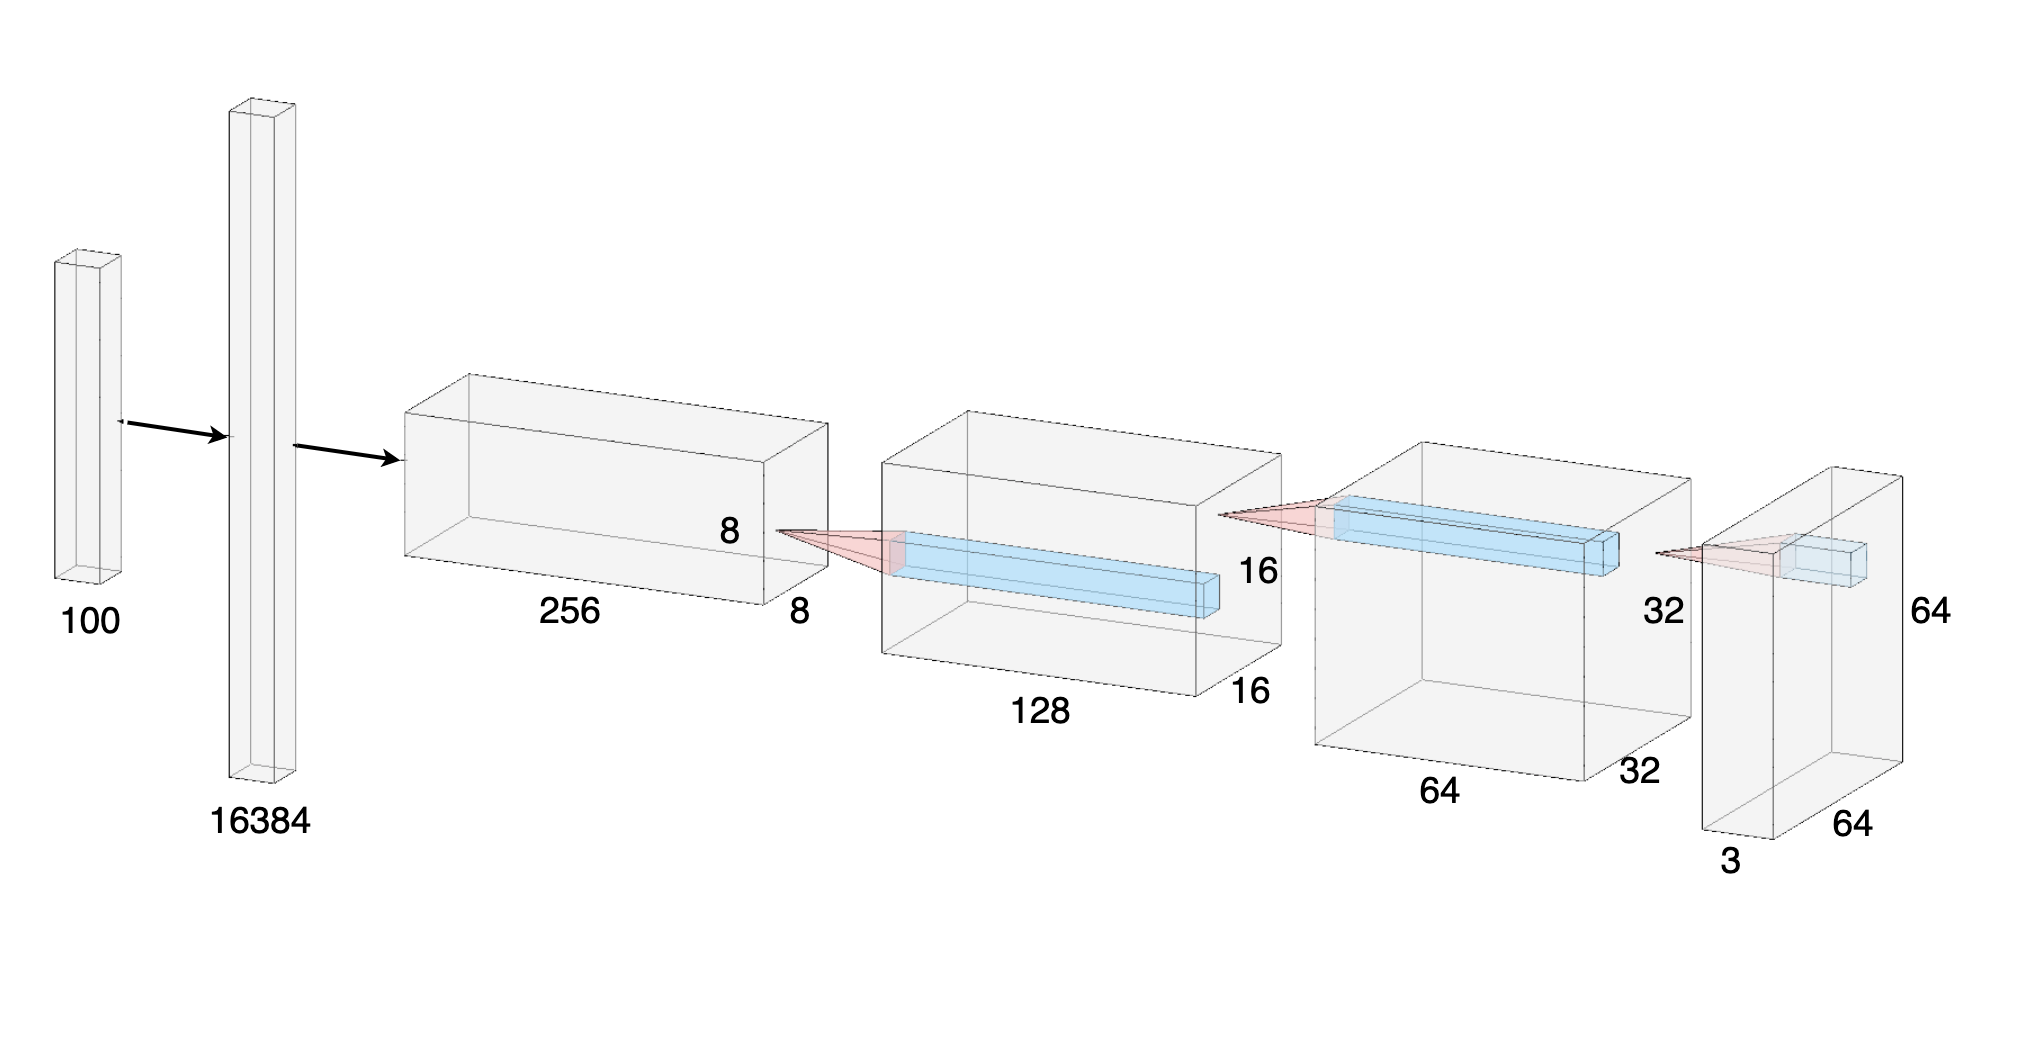
\includegraphics[scale=0.12]{gen.png}
	\caption[center]{Architektur des Generators $G$ }
	\label{fig:gen}
\end{figure}


\section{Implementierungsdetails}
Das entworfene Konzept wurde mit der \emph{TensorFlow}-API \cite{tensorflow2015-whitepaper} in Python implementiert. Unterstützend wurde die \emph{TensorFlow Dataset}-API eingesetzt um die Trainingsdaten einzulesen und um die in Abschnitt \ref{sec:2} beschriebenen Vorbereitungsschritte umzusetzen.  Das entworfene Netzwerk wurde in einer Online-Entwicklungsumgebung auf kaggle\footnote{\url{www.kaggle.com}} implementiert. Kaggle bietet die Möglichkeit, die Berechnungen mit der Hilfe von GPUs und Tensor Processing Units (TPUs) zu beschleunigen. Das GAN wurde innerhalb von 150 Epochen mit einer Batch Size von 128 trainiert. Als \emph{Optimizer} wurde das Adam-Verfahren \cite{kingma2014method} gewählt.

\section{Ergebnisse}
Die Ergebnisse nach 150 Epochen können in Abbildung \ref{fig:result} gesehen werden. Der Generator hat offensichtlich während des Trainings gelernt, wie menschliche Gesichter aussehen und ist in der Lage, anhand eines Zufallsvektors $X_{random}$, neue Bilder von Gesichtern zu generieren.

\section{Fazit}
In der vorliegenden Arbeit konnte mit relativ geringem zeitlichen Aufwand ein GAN zur Erstellung von Bildern mit menschlichen Gesichtern implementiert werden. Eine Verbesserung des Ergebnisses durch eine ausgefeiltere Wahl der Hyperparameter ist noch offen.

\bibliographystyle{asmems4}

% Here's where you specify the bibliography database file.
% The full file name of the bibliography database for this
% article is asme2e.bib. The name for your database is up
% to you.
\bibliography{asme2e}

\end{document}
